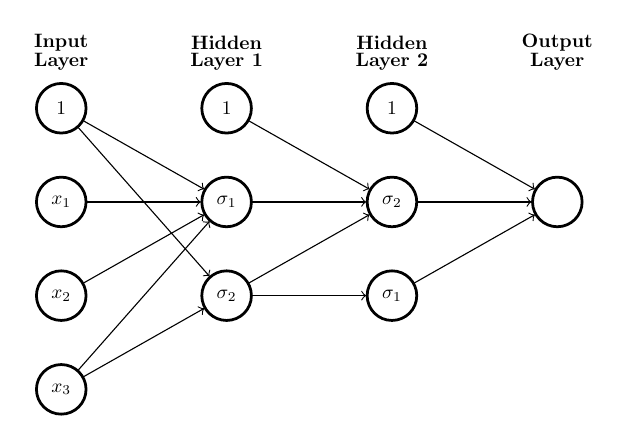
\begin{tikzpicture}[scale=0.7, every node/.style={scale=0.7}]
    %--------------------%
    % Parameters
    %--------------------%
    \def\layersep{3}
    \def\ysep{1.7}
    \def\circlesize{0.9cm}
    \def\labelshift{0.75}
    \def\woffset{5}
    \def\linethic{1.0pt}

    %--------------------%
    % Input Layer
    %--------------------%

    \node[draw, circle, minimum size=\circlesize, line width=\linethic] (theta0) at (0,2*\ysep) {1};
    \node[draw ,circle, minimum size=\circlesize, line width=\linethic] (x1) at (0,1*\ysep) {$x_1$};
    \node[draw ,circle, minimum size=\circlesize, line width=\linethic] (x2) at (0,0*\ysep) {$x_2$};
    \node[draw ,circle, minimum size=\circlesize, line width=\linethic] (x3) at (0,-1*\ysep) {$x_3$};

    %--------------------%
    % Layer 1
    %--------------------%
    % Nodes
    \node[draw, circle, minimum size=\circlesize, line width=\linethic] (theta1) at (\layersep,2*\ysep) {1};
    \node[draw ,circle, minimum size=\circlesize, line width=\linethic] (node11) at (\layersep,1*\ysep) {$\sigma_{1}$};
    \node[draw ,circle, minimum size=\circlesize, line width=\linethic] (node12) at (\layersep,0*\ysep) {$\sigma_{2}$};

    %--------------------%
    % Layer 2
    %--------------------%
    % Nodes
    \node[draw ,circle, minimum size=\circlesize, line width=\linethic] (theta2) at (2*\layersep,2*\ysep) {1};
    \node[draw ,circle, minimum size=\circlesize, line width=\linethic] (node21) at (2*\layersep,1*\ysep) {$\sigma_{2}$};
    \node[draw ,circle, minimum size=\circlesize, line width=\linethic] (node22) at (2*\layersep,0) {$\sigma_{1}$};

    %--------------------%
    % Output Layer
    %--------------------%
    \node[draw ,circle, minimum size=\circlesize, line width=\linethic] (out) at (3*\layersep,1*\ysep) {};

    %--------------------%
    % Connections
    %--------------------%
    % Input to Layer 1
    \draw[->] (theta0) -- node[above,midway]{} (node11);
    \draw[->] (theta0) -- node[above,midway]{} (node12);
    \draw[->] (x1) -- node[above,midway]{} (node11);
    %\draw[->] (x1) -- node[above,midway]{} (node12);
    \draw[->] (x2) -- node[above,midway]{} (node11);
    %\draw[->] (x2) -- node[above,midway]{} (node12);
    \draw[->] (x3) -- node[above,midway]{} (node11);
    \draw[->] (x3) -- node[above,midway]{} (node12);

    % Layer 1 to Layer 2
    \draw[->] (theta1) -- node[above,midway]{} (node21);
    %\draw[->] (theta1) -- node[above,midway]{} (node22);
    \draw[->] (node11) -- node[above,midway]{} (node21);
    %\draw[->] (node11) -- node[above,midway]{} (node22);
    \draw[->] (node12) -- node[above,midway]{} (node21);
    \draw[->] (node12) -- node[above,midway]{} (node22);

   % Layer 2 to Output Layer
    \draw[->] (theta2) -- node[above,midway]{} (out);
    \draw[->] (node21) -- node[above,midway]{} (out);
    \draw[->] (node22) -- node[above,midway]{} (out);


    %--------------------%
    % Layer Labels
    %--------------------%
    \node at (0*\layersep, 2.7*\ysep) {\textbf{Input}};
    \node at (0*\layersep, 2.5*\ysep) {\textbf{Layer}};
    \node at (1*\layersep, 2.7*\ysep) {\textbf{Hidden}};
    \node at (1*\layersep, 2.5*\ysep) {\textbf{Layer 1}};
    \node at (2*\layersep, 2.7*\ysep) {\textbf{Hidden}};
    \node at (2*\layersep, 2.5*\ysep) {\textbf{Layer 2}};
    \node at (3*\layersep, 2.7*\ysep) {\textbf{Output}};
    \node at (3*\layersep, 2.5*\ysep) {\textbf{Layer}};

\end{tikzpicture}
